\subsection{Deep Learning}
    \framepic{graphics/deeplearning/deep-learning}{
        \framefill
        \textcolor{white}{Deep Learning}
        \vskip 0.5cm
    }

    \begin{frame}{Computer Vision}
        \begin{block}{Classification Task}
            To determine to which of a set of \textbf{categories} a given object belongs to.
        \end{block}
        \begin{columns}[onlytextwidth]
            \column{0.3\textwidth}
            \centering
            \includegraphics[width=\textwidth]{graphics/computervision/classification-image.jpeg}
            \onslide <2-> {
                \column{0.4\textwidth}
                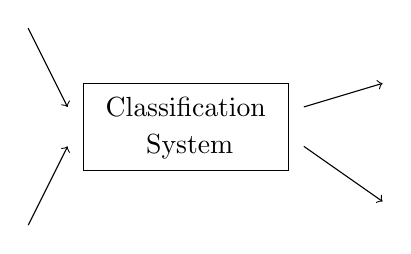
\begin{tikzpicture}
                    \node at (0,0) {Classification};
                    \node at (0.05,-0.5) {System};
                    \node[rectangle, draw, minimum width=2.6cm, minimum height=1.1cm, anchor=north west] at (-1.3,0.3) {};
                    \draw[->] (-2,1) -- (-1.5,0);
                    \draw[->] (-2,-1.5) -- (-1.5,-0.5);
                    \onslide <3-> {
                        \draw[->] (1.5,0) -- (2.5,0.3);
                        \draw[->] (1.5,-0.5) -- (2.5,-1.2);
                    }
                \end{tikzpicture}
            }
            \onslide <3-> {
                \column{0.2\textwidth}
                \vskip -0.5cm Output \vskip 0.5cm
                \begin{columns}[onlytextwidth]
                    \column{0.5\textwidth}
                        \begin{tabular}{|c|}
                            \hline
                            $0.03$\\\hline
                            \cellcolor{UniBlue}\textcolor{white}{$0.77$}\\\hline
                            $\vdots$\\\hline
                            $0.12$\\\hline
                        \end{tabular}
                    \column{0.5\textwidth}
                        \vskip -0.2cm
                        \begin{tabular}{c}
                            \\
                            \textcolor{UniBlue}{Child}\\
                            \\
                            \\
                        \end{tabular}
                \end{columns}
            }
        \end{columns}
    \end{frame}

    \begin{frame}{Computer Vision}
        \begin{block}{Object Localization Task}
            To find a given number (usually one) of items in a given context, predicting both their position and their class. \\
            \textbf{Remark.} Position is usually given as a bounding box.
        \end{block}
        \begin{columns}[onlytextwidth]
            \column{0.45\textwidth}
            \onslide <2-> {
                \includegraphics[width=\textwidth]{graphics/computervision/localization-input}
            }
            \column{0.45\textwidth}
            \onslide <3-> {
                \includegraphics[width=\textwidth]{graphics/computervision/localization-output}
            }
        \end{columns}
    \end{frame}

    \begin{frame}{Computer Vision}
        \onslide<1-> {
            \begin{block}{Object Detection Task}
                To \textbf{localize} any number of items in a given context, allowing either zero or any finite number of objects.
            \end{block}
        }
        \onslide<2-> {
            \begin{alertblock}{Remark.}
                The constraint on the number of object is \emph{a priori}. Indeed, a localization system will always look for a fixed number of objects, whereas a detection system is trained to be able to spot a variable number of objects in each input.
            \end{alertblock}
        }
    \end{frame}

    \begin{frame}{Computer Vision}
        \onslide <1-> {
            \begin{block}{Image Segmentation}
                Pixel-wide classification of the image. \textbf{Remark.} Image segmentation can be consider either the preemptive step to classification or the output of a classification system.
            \end{block}
        }
        \onslide <2-> {
            \vskip -0.5cm 
            \begin{exampleblock}{Example: Pixel-based image segmentation.}
                This family considers some distance defined over the image domain to segmentate it.
            \end{exampleblock}
        }
        \onslide <3-> {
            \vskip -0.5cm 
            \begin{exampleblock}{Example: Edge-based image segmentation.}
                This family uses an edge-detector algorithm, along with denoising and thresholding considerations, to solve the boundary detection problem.
            \end{exampleblock}
        }
    \end{frame}

    \begin{frame}{Training}
        \begin{block}{Forward propagation}
            The \emph{feedforward} neural network accepts an input $\underline{\underline{X}}$ and produce an output $\underline{y}$. The information from $\underline{\underline{X}}$ flows through the hidden units to produce $\underline{y}$. This is called \textbf{forward propagation}.
        \end{block}

        \begin{block}{Backward propagation}
            During the training the forward propagation can continue onward to evaluate a scalar cost $J\left(\underline{\underline{\theta}}\right)$. The \textbf{back-propagation} algorithm is a numerically efficient way to compute cost gradient, in order to perform gradient descent.
        \end{block}    
    \end{frame}

    \begin{frame}{Deep Learning}
        \includegraphics[width=\textwidth]{graphics/deeplearning/nn}
    \end{frame}

    \begin{frame}
        \frametitle{Training}
        \framesubtitle{Backpropagation (proof)}
        \centering
        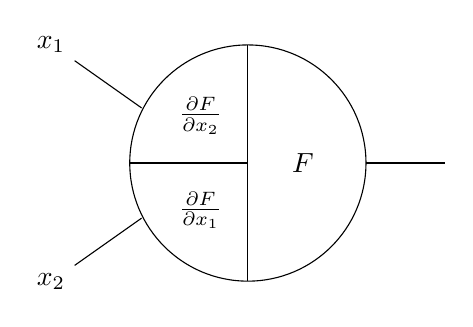
\begin{tikzpicture}
            \node[circle, draw, minimum width=3cm, minimum height=3cm] at (0,0) {};
            \node at (0.7,0) {$F$};
            \node at (-0.6,-0.6) {$\frac{\partial F}{\partial x_1}$};
            \node at (-0.6,0.6) {$\frac{\partial F}{\partial x_2}$};
            \node at (-2.5,1.5) {$x_1$};
            \node at (-2.5,-1.5) {$x_2$};

            \draw (0,0) -- (-1.5,0);
            \draw (0,-1.5) -- (0,1.5);
            \draw (1.5, 0) -- (2.5,0);

            \draw (-1.35, 0.7) -- (-2.2,1.3);
            \draw (-1.35, -0.7) -- (-2.2,-1.3);
        \end{tikzpicture}

        \vskip 0.5cm
        
        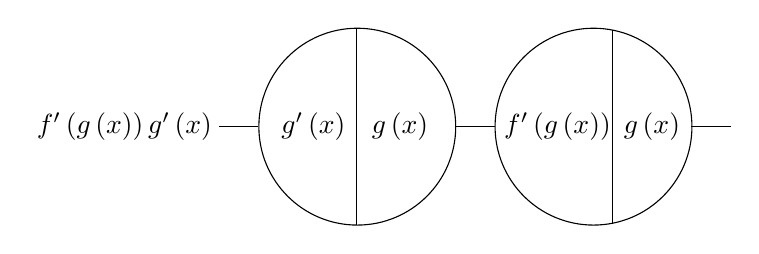
\begin{tikzpicture}
            \node at (-.7,0) {$f'\left(g\left(x\right)\right)g'\left(x\right)$};

            \draw (0.5,0) -- (1,0);

            \node[circle, draw, minimum width=2.5cm, minimum height=2.5cm, anchor=west] at (1,0) {};
            \node at (1.7, 0) {$g'\left(x\right)$};
            \node at (2.8, 0) {$g\left(x\right)$};
            \draw (2.25, 1.25) -- (2.25, -1.25);

            \draw (3.5, 0) -- (4, 0);

            \node[circle, draw, minimum width=2.5cm, minimum height=2.5cm, anchor=west] at (4,0) {};
            \node at (4.8, 0) {$f'\left(g\left(x\right)\right)$};
            \node at (6, 0) {$g\left(x\right)$};
            \draw (5.5, 1.23) -- (5.5, -1.23);

            \draw (6.5, 0) -- (7, 0);

        \end{tikzpicture}
    \end{frame}

    \begin{frame}{Convolutional Networks}
        \includegraphics[width=\textwidth]{graphics/deeplearning/cnn}
        \vskip 0.5cm
        \begin{exampleblock}{Motivation}
            \begin{enumerate}
                \item Sparse interactions
                \item Parameter sharing
                \item Equivariant representations
                \item Biologically inspired artificial intelligence
            \end{enumerate}
        \end{exampleblock}
    \end{frame}

    \begin{frame}{Convolutional Networks}
        \includegraphics[width=\textwidth]{graphics/deeplearning/cnn}
        \onslide <1-> {
            \begin{block}{Convolutional neural networks (CNN)}
                CNNs are a specialized kind of neural network for processing data that has a known grid-like topology.
            \end{block}
        }
        \onslide <2-> {
            \begin{block}{Convolutional neural networks (CNN) - 2}
                CNNs are neural networks that use convolution in place of general matrix multiplication in at least one of their layers.
            \end{block}
        }
    \end{frame}